\documentclass[10pt]{beamer}

\usepackage[utf8]{inputenc}
\usepackage{tcolorbox}
\usepackage{tikz}
\usetikzlibrary{intersections,calc}
\usepackage{amsmath}
\usepackage{graphicx}
\def \heart {\textcolor{blue}{$\heartsuit$} }
\def \C {$\mathcal{C}$}



\tcbset{%
	basic/.style={colframe=black,
		      colback=white,
		      top= 0mm,
		      bottom = 2mm,
		      boxsep=0mm
		      }
}

\begin{document}  
    \beamertemplatenavigationsymbolsempty
    
    \frame{ % énoncé ex1
	  
	  \frametitle{Q1 Juillet 2016.} 
	  
	  
	  Par un point $P$ intérieur à un cercle $\mathcal{C}$ de centre $O$ et de rayon $r$, on
	  mène deux droites perpendiculaires $d_1$ et $d_2$ . On note $A_1$ un des points
	  d’intersection de $d_1$ avec $\mathcal{C}$, et $A_2$ un des points d’intersection de $d_2$
	  avec $\mathcal{C}$. Le milieu de la corde $[A_1 A_2 ]$ est noté $M$ . Démontrer l’égalité
	  $$ |OM|^2 + |PM|^2 = r^2,$$
	  où $|XY|$ dénote la longueur du segment $[XY]$.
	  
	  \vfill
	  
	  \pause
	  % hypothèses et thèse
	  \begin{tcolorbox}[basic] 
	      \begin{columns}[t]
		 
		 \column{.5\textwidth}\centering
		      
		      \underline{Hypothèses} 
		      \begin{itemize}
		      \item $d_1 \bot d_2$,
		      \item $|A_1M|=|MA_2|$.
		      \end{itemize}

		  
		  \column{.5\textwidth}\centering
		      
		      \underline{Thèse} \\
		      \smallskip
		      $ |OM|^2 + |PM|^2 = r^2$.
		
	      \end{columns}
	  \end{tcolorbox}
	  
    }
    
    \frame{ % résolution ex1
	  \begin{columns}[t]
		\column{.5\textwidth}\centering 
		

			\underline{Dessin}\\
			
				  \begin{figure}[h]
				  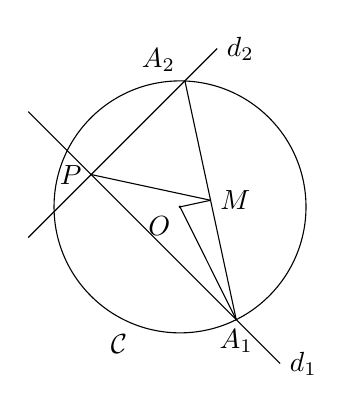
\begin{tikzpicture}[scale=0.8]
					%\draw[help lines] (-3,-3) grid (3,3); 
					
					%CERCLE
					\coordinate[label=below left:$O$] (O) at (0,0);
					\fill (O) circle (0.025);
					\draw[name path=cercle] (O) circle (2cm);
					\node[below left] (C) at (-110:2) {$\mathcal{C}$};
					
					% P
					\coordinate[label=left:$P$] (P) at (160:1.5);
					
					%D_1 et D_2
					\draw[name path=d_1] (P) -- +(3,-3) node[right]() {$d_1$};
					\draw (P) -- +(-1,1);
					\draw[name path=d_2] (P) -- +(2,2) node [right]() {$d_2$};
					\draw (P) -- +(-1,-1);
							
					%A_1,A_2 et M 
					\path [name intersections={of=d_1 and cercle,by=A_1}];
					\node [below] at (A_1) {$A_1$};
					\path [name intersections={of=d_2 and cercle,by=A_2}];
					\node [above left] at (A_2) {$A_2$}; 
					\draw (A_1) -- (A_2) coordinate[pos=0.5,label=right:$M$](M);
					
					
					%segments [PM],[OM],[OA_1]
					\draw (P) -- (M);
					\draw (O) -- (A_1);
					\draw (O) -- (M);
				  \end{tikzpicture}
				  \end{figure}
			
				  \begin{tcolorbox}[basic] 
				      
				    \smallskip
				    \underline{Hypothèses} 
				    \begin{enumerate}
				    \item  $d_1 \bot d_2$,
				    \item  $|A_1M|=|MA_2|$.
				    \end{enumerate}
							      
				    \underline{Thèse} \\
				    \smallskip
				    $ |OM|^2 + |PM|^2 = r^2$.
				    \end{tcolorbox}
		
		
		\column{.5\textwidth}\centering
		
		\underline{Résolution}\\
		
		\begin{enumerate}
		 \item $\Delta A_1A_2P$ rectange,
		 \item $[PM]$ médiane du $\Delta A_1A_2P$. 
		\end{enumerate}
		
		\begin{itemize} 
		\item[$\heartsuit$]La longueur de la médiane issue de l'angle droit d'un $\Delta$ rectange vaut la moitié de celle de l'hypothénuse.
		\end{itemize}
		
		$|PM| = |MA_1|$ \\
		\medskip 
		\flushleft Thèse : $|OM|^2 + |MA_1|^2 = r^2$\\	\centering
		$i.e.$ $\Delta OMA_1$ est rectange. \\
		
		\begin{itemize} 
		\item[$\heartsuit$]La droite passant par le centre d'un cercle et le milieu d'une de ses cordes est perpendiculaire à cette dernière.
		\end{itemize}
		
		$OM \bot A_1A_2$ \\
		\medskip 
		\hfill $\Delta OMA_1$ est rectange. \hfill $\qed$

   
	   \end{columns}
	   }
	 
  \frame{ % énoncé ex2
	
	\frametitle{Q2 Juillet 2016.} 
	  
	  On donne une droite $d$ tangente à un cercle $\mathcal{C}$, et on considère le lieu
	  des points dont la distance à $\mathcal{C}$ est égale à la distance à $d$. On demande
	  de caractériser ce lieu à l’aide d’équations cartésiennes, de préciser la
	  nature de celui-ci, et de le représenter graphiquement.
	  	  
	  \vfill
	  
	  \pause	  
	  % Conditions
	  \begin{tcolorbox}[basic] 
	      \begin{columns}[t]
		 
		 \column{.5\textwidth}\centering
		      
		      \underline{Procédé} \\
		      \begin{itemize}
		       \item Poser un repère orthonormé,
		       \item Exprimer la condition pour qu'un point $P$ appartienne au lieu.
		      \end{itemize}
		   		  
		  \column{.5\textwidth}\centering
		      
		      \underline{Condition} \\
		      \bigskip
		       $\mathcal{D}(P,d) = \mathcal{D}(P,\mathcal{C})$.
		      

		
	      \end{columns}
	  \end{tcolorbox}
	  	  
	}
	
  \frame{ %Résolution
	
	\begin{columns}[t]
		\column{.5\textwidth}\centering 
		

			\underline{Dessin}\\
			
				  \begin{figure}[h]
				  \begin{tikzpicture}[scale=0.8]
					%\draw[help lines] (-3,-3) grid (3,3); 
					
					%AXES
					\draw[->] (0,-3) -- (0,3) coordinate[label=below right:$y$]();
					\draw[->] (-3,0) -- (3,0) coordinate[label=above left:$x$]();
					%CERCLE									
					\draw (0,0) circle (1.5cm);
					\node[below left] (C) at (110:2) {$\mathcal{C}$};
					\coordinate[label=above:$r$] () at (1.5/2,0);
					%DROITE D
					\draw (-3,-1.5) coordinate[label= below right:$d$]() -- (3,-1.5); 
					%Point P
					\coordinate[label=above:$P$] (P) at (-30:2);
					\draw (P) circle (0.025cm);
					

				
				  \end{tikzpicture}
				  \end{figure}
			\begin{tcolorbox}[basic]
			\smallskip
			\centering
			\underline{Condition} \\
		        \smallskip
		        $\mathcal{D}(P,d) = \mathcal{D}(P,\mathcal{C})$.	  
			\end{tcolorbox}
			
		\column{.5\textwidth}\centering
		
		\underline{Résolution}\\
		Soit un repère orthonormé $R=(O,X,Y)$ avec :
		\begin{itemize}
		 \item[$\bullet$] $P (x,y)$,
		 \item[$\bullet$] $\mathcal{C} \equiv x^2 + y ^2 = r^2$,
		 \item[$\bullet$] $d \equiv y = -r$.
		\end{itemize}
		
		\begin{enumerate}
		 \item $\mathcal{D}(P,d) = |y+r|$ \\ Distance entre $P$ et sa projection orthogonale sur $d$. 
		 \item $\mathcal{D}(P,\mathcal{C}) = |\sqrt{x^2+y^2}-r|$ \\ Distance entre $P$ et sa projection orthogonale sur $\mathcal{C}$.
		\end{enumerate}
		
		\bigskip
		$|y+r| = |\sqrt{x^2+y^2}-r|$ \\
		
	\end{columns}
  
	}
  
  \frame{%Résolution
	 \centering
	 \bigskip
	 $|y+r| = |\sqrt{x^2+y^2}-r|$ \medskip
	 \begin{columns}[t]
	  \column{.5\textwidth}\centering
	  Pour :
	  \begin{itemize}
	   \item $P$ au-dessus de $d$ et $P$ à l'extérieur du cercle, ou
	   \item $P$ en dessous de $d$ et $P$ à l'intérieur du cercle (imp.).
	  \end{itemize}
	  
	  $y+r = \sqrt{x^2+y^2}-r$ \\ \bigskip

	  $y=\dfrac{x^2}{4r}-r$ $(r\neq0)$.\\
	  
	  

	  \column{.5\textwidth}\centering
	  Pour :
	  \begin{itemize}
	   \item $P$ au-dessus de $d$ et $P$ à l'intérieur du cercle, ou
	   \item $P$ en dessous de $d$ et $P$ à l'extérieur du cercle.
	  \end{itemize}
	  
	  $y+r = -\sqrt{x^2+y^2}+r$ \\ \bigskip \medskip
	  $x=0$ et $y\leq0$. \\
	  
	 \end{columns}
	
	
	\underline{Dessin}\\
			
				  \begin{figure}[h]
				  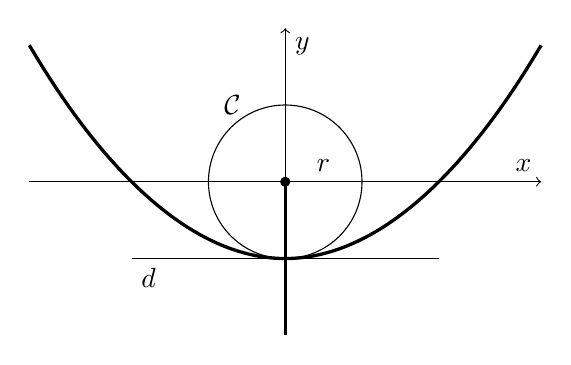
\begin{tikzpicture}[scale=0.65]
					%\draw[help lines] (-3,-3) grid (3,3); 
					
					%AXES
					\draw[->] (0,-3) -- (0,3) coordinate[label=below right:$y$]();
					\draw[->] (-5,0) -- (5,0) coordinate[label=above left:$x$]();
					%CERCLE									
					\draw (0,0) circle (1.5cm);
					\node[below left] (C) at (110:2) {$\mathcal{C}$};
					\coordinate[label=above:$r$] () at (1.5/2,0);
					%DROITE D
					\draw (-3,-1.5) coordinate[label= below right:$d$]() -- (3,-1.5); 
					%LIEU
					\fill (0,0) circle (0.1);
					\draw[very thick] (0,0) -- (0,-3);
					\draw[very thick] (-5,2.66667) parabola bend(0,-1.5) (5,2.66667);
					
				  \end{tikzpicture}
				  \end{figure}

	
  
	}
  
	  
	  
\end{document}
